\documentclass[a4paper,10pt,ngerman]{scrartcl}
\usepackage{babel}
\usepackage[T1]{fontenc}
\usepackage[utf8x]{inputenc}
\usepackage[a4paper,margin=2.5cm,footskip=0.5cm]{geometry}
\usepackage{float}
\usepackage{subfigure}
\usepackage{wrapfig}

% Die nächsten drei Felder bitte anpassen:
\newcommand{\Aufgabe}{Aufgabe 5: Hüpfburg} % Aufgabennummer und Aufgabennamen angeben
\newcommand{\TeilnahmeId}{66432}                  % Teilnahme-ID angeben
\newcommand{\TeamId}{00662}
\newcommand{\Name}{Linus Schumann}             % Name des Bearbeiter / der Bearbeiterin dieser Aufgabe angeben

% Kopf- und Fußzeilen
\usepackage{scrlayer-scrpage, lastpage}
\setkomafont{pageheadfoot}{\large\textrm}
\lohead{\Aufgabe}
\rohead{Teilnahme-ID: \TeilnahmeId, L. Schumann}
\cfoot*{\thepage{}/\pageref{LastPage}}

% Position des Titels
\usepackage{titling}
\setlength{\droptitle}{-1.0 cm}

% Für mathematische Befehle und Symbole
\usepackage{amsmath}
\usepackage{amssymb}

% Für Bilder
\usepackage{graphicx}

% Für Algorithmen
\usepackage{algpseudocode}

% Für Quelltext
\usepackage{listings}
\usepackage{color}
\definecolor{mygreen}{rgb}{0,0.6,0}
\definecolor{mygray}{rgb}{0.5,0.5,0.5}
\definecolor{mymauve}{rgb}{0.58,0,0.82}
\lstset{
  keywordstyle=\color{blue},commentstyle=\color{mygreen},
  stringstyle=\color{mymauve},rulecolor=\color{mygray},
  basicstyle=\footnotesize\ttfamily,numberstyle=\tiny\color{mygray},
  captionpos=b, % sets the caption-position to bottom
  keepspaces=true, % keeps spaces in text
  numbers=left, numbersep=5pt, showspaces=false,showstringspaces=true,
  showtabs=false, stepnumber=2, tabsize=2,
  breaklines=true,
  frame=lines,
  framesep=10pt,
  postbreak=\mbox{\textcolor{red}{$\hookrightarrow$}\space}
}

% Anklickbare Links im Dokument
\usepackage{hyperref}
\usepackage{cleveref}
\hypersetup{
    colorlinks,
    citecolor=black,
    filecolor=black,
    linkcolor=black,
    urlcolor=black
}

% Daten für die Titelseite
\title{\textbf{\Huge\Aufgabe}}
\author{\LARGE Teilnahme-ID: \LARGE \TeilnahmeId \\\\
      \LARGE Team-ID: \LARGE \TeamId \\\\
	    \LARGE Bearbeiter/-in dieser Aufgabe: \\ 
	    \LARGE \Name\\\\}
\date{\LARGE\today}

%% ___ Anfang ___ %%
\begin{document}
  \maketitle
  \tableofcontents
  \vspace{6cm}

  %% ___ Lösungsidee ___ %%
  \section{Lösungsidee\label{sec:Loesungsidee}}
    \subsection{Feststellung des Problems}
      Das Problem bei dieser Aufgabe liegt darin, dass Sasha und Mika gleichzeitig auf dem selben Feld laden sollen. Sasha startet auf Feld 1 ($x_{1}$) und Mika auf Feld 2 ($x_{2}$). Sie bewegen sich auf einem Parcour, der als ungewichteter gerichteter Graph dargestellt werden kann. Die Anzahl an Knoten wird im Folgenden immer als $n$ und die Anzahl an Kanten immer als $m$ bezeichnet. Für $n$ gilt $2 \leq n \leq 150$ und für $m$ gilt $1 \leq m \leq 347$. Dies lässt sich dem größten Beispiel (\cref{sec:Beispiele:2}) entnehmen. Die Knoten sind von 1 bis n durchnummeriert und werden immer als $x_{i}$ (mit $1 \leq i \leq n$) bezeichnet. Auffällig ist dabei, dass $n$ nicht sehr groß ist und es daher wahrscheinlich keine sehr schnelle Lösung gibt, da es sonst größere Beispiele geben würde.
      \\
      Außerdem muss im Folgenden beachtet werden, dass der Graph mehr als $n-1$ Kanten hat und damit keine Baumstruktur aufweißt. Daher können im Graphen Zyklen enthalten sein. Auch gibt es keine Einschränkung zur mehrfachen Nutzung von Knoten innerhalb eines Pfades.
    \subsection{Erste Idee\label{sec:Loesungsidee:1}}
      Die erste Idee um dieses Problem nun zu lösen, besteht darin von beiden Startknoten ($x_{1}$ und $x_{2}$) aus alle möglichen Pfade zu jedem anderen Knoten zu finden. Dannach kann man dann die Länge der Pfade vergleichen und bei gleicher Länge beide Pfade ausgeben. Es kann dabei allerdings Pfade geben in denen ein bestimmter Knoten nur mit der passenden Distanz erreicht werden kann, wenn Knoten mehrfach genutzt werden. Dies funktiert da der Graph zyklisch sein kann. Daher kann die Idee nicht mit einer einfachen Tiefensuche implementiert werden, die den aktuellen Pfad speichert, da kein Abbruch Kriterium definiert wäre. Bei einer ''normalen'' Tiefensuche würde dazu Vector genutzt werden, in denen die bereits besuchten Knoten gespeichert werden würden.
      \\
      Durch diese Vorraussetzungen ist die intuitivste Abbruchbedingung eine maximale Tiefe $tMax$ zu definieren, die ein Pfad maximal lang sein darf.
    \subsection{Optimierung dieser Idee}
      Da diese Lösung vor allem für längere Pfade sehr sehr langsam ist, macht es Sinn über eine mögliche Optimierung nachzudenken.
      \\
      Diese Optimierung besteht darin, dass man für jeden Startknoten ($x_{1}$ und $x_{2}$), eine dreidimensionale Matrix erstellt. Diese beiden Matritzen werden nun $a$ und $b$ genannt. In dieser wird für jeden anderen Knoten für jede Distanz (bis zur maximalen Distanz) ein Pfad als Vector gespeichert. Dabei befindet sich der Pfad Vector zum Knoten $i$ (für $1 \leq i \leq n$) mit der Länge $j$ (für $1 \leq j \leq tMax$) an der Stelle $a_{i,j}$.
      \\Beim Starten des Algorithmus ist wird die Matrix $a$ und $b$ mit leeren Vectoren für $a_{i,j}$ erstellt. Dann kann die Tiefensuche aus der ersten Idee (\cref{sec:Loesungsidee:1}) für beide Startknoten genutzt werden. Dabei wird bei jedem Schritt der Tiefensuche überprüft, ob schon ein Pfad zu diesem Knoten $x_{i}$ und mit der selben Länge {t} gegeben ist. Nur wenn es noch keinen Vector in $a$ bzw. $b$ an der Stelle $a_{i,t}$ bzw. $b_{i,t}$ gibt, wird der aktuelle Pfad an dieser Stelle gespeichert. Dadurch werden keine doppelten Pfade berechnet und die Laufzeit wird deutlich verbessert.
    \subsection{Finden der kürzesten Pfade}
      Am Schluss hat man durch die Verwendungung der beiden Matritzen außerdem den Vorteil, dass man direkt die minimalen Pfade herausfinden kann. Dazu werden die beiden Matritzen so verglichen, dass für eine Distanz $t$ ($1 \leq t \leq tMax$) zuerst jeder Endknoten $x_{i}$ ($1 \leq i \leq n$) überprüft wird und danach erst die Distanz erhöht wird. Falls also $|a_{i,t} > 0|$ und $|b_{i,t} > 0|$ gilt, wurde eine Lösung gefunden, da falls es einen Pfad an der Stelle $i,t$ gibt $|a_{i,t}| = t$ und $|b_{i,t}| = t$ gilt.
      

  %% ___ Umsetzung ___ %%
  \section{Umsetzung\label{sec:Umsetzung}}
    \subsection{Allgemeines}
      Im Folgenden wird die Umsetzung der in \cref{sec:Loesungsidee} beschriebene Lösungsidee, näher erläutert.  Grundsätzlich wurde diese Idee dabei in C++, genauer gesagt in der Datei ''Aufgabe\_5.cpp'' implementiert. Diese Datei befindet sich im Verzeichnis ''./source/''.
      \\\\
      Um das implementierte Programm zu starten kann das Batch Skript ''Aufgabe\_5.bat'' im Verzeichnis ''./executables/'' genutzt werden. Dieses startet das von mir für Windows kompilierte Programm (''Aufgabe\_5.exe''). Für andere Betriebssysteme müsste die Source-Datei erneut auf dem entsprechenden Rechner kompiliert werden.
      \\\\
      Im Verzeichnis ''./beispieleingaben/'' befinden sich alle in dieser Dokumentation aufgeführten Beispiele und im Verzeichnis ''./beispielausgaben/'' befinden sich dementsprechend die gesicherten Ausgaben.
      Letztere werden mit der Datei-Endung ''.out'' gespeichert. Außerdem werden bei jeder Ausgabe auch noch zwei ''.dot'' und zwei ''.png'' Dateien gespeichert. Näheres zu diesen Dateien wird in \cref{sec:Umsetzung:Visualisierung} (Visualisierung) genannt.

    \subsection{Implementation der Lösungsidee}
      Nun werden die einzelnen Bestandteile der Implementation näher erläutert.
      \subsubsection{Einlesen des Graphen}
        Im ersten Schritt der Implementation wird der Graph aus der Eingabedatei eingelesen. Um den Graph zu speichern, wird eine Adjazenzliste verwendet. Dabei wird für jeden Knoten eine Liste mit den Nachbarknoten erstellt.\\
        Im Vergleich zur Adjazenzmatrix bringt dies den Vorteil, dass die Speicherkomplexität deutlich geringer ist. Genauer gesagt liegt diese bei der Adjazenzliste bei $\mathcal{O}(n + m)$ und bei der Adjazenzmatrix würde diese bei $\mathcal{O}(n^2)$ liegen.
      \subsubsection{Für jede Distanz Pfade finden}
        Nach dem Einlesen des Graphen wird wie in der Lösungsidee beschrieben zwei mal eine Tiefensuche ausgeführt, die alle Pfade im Graphen findet, die beim Knoten 0 bzw. 1 starten. Dies wurde in der Funktion ''dfs'' implementiert. Um diese Tiefensuche zu implementieren wird jeweils eine ''Pfade'' Matrix erstellt, der für jeden Knoten alle Pfade mit unterschiedlichen Distanzen speichert. Bei jedem Aufruf der Funktion wird dazu geprüft, ob schon ein Pfad mit dieser Länge zu diesem Knoten in dem ''Pfad'' Vektor gespeichert ist.\\
        Außerdem muss die Funktion natürlich immer den aktuellen Pfad speichern, dazu wird ein positiver Effekt der Rekursion genutzt. Der Pfad wird nämlich in einem Vektor gespeichert, der bei jedem Aufruf der Funktion als Referenz übergeben wird. Die Rekursion bietet dann den Vorteil, dass zuerst der aktuelle Knoten an das Ende des Vektor gehängt wird. Dann wird die Funktion für alle Nachbarknoten aufgerufen und danach der aktuelle Knoten wieder aus dem Vektor entfernt wird. Aus diesem Grund ist der Pfad immer aktuell.
      \subsubsection{Gleiche und kürzeste Pfade finden}
        Nach dem Füllen der beiden ''Pfade'' Matritzen können diese ausgewertet werden. Dazu werden zwei for-Schleifen genutzt. Die Erste iteriert über alle Distanzen und die zweite über alle Knoten. Wenn zwei Pfade an der selben Stelle gefunden werden, wurde die beste Lösung gefunden und die Schleifen werden unterbrochen.\\\\
        Dieser Schritt hat auf Grund der zwei for-Schleifen eine maximale Laufzeit von $\mathcal{O}(1000 * n)$ (Die 1000 würden theoretisch wegfallen).
    \subsection{Visualisierung\label{sec:Umsetzung:Visualisierung}}
      Um die unterschiedlichen Graphen zu visualiseren wurde das Programm Graphviz genutzt. Dieses muss auf dem ausführenden System installiert sein, da sonst kein PNG-Bild generiert werden kann. Dazu wird nämlich am Ende der main-Funktion zweimal der Befehl ''dot'' aufgerufen, um aus den beiden vorher generierten ''.dot'' Dateien ein Bild zu machen.\\\\
      Diese beiden ''.dot'' Dateien werden vorher im Programm generiert und beschreiben einfach den Aufbau des Graphen. Dabei wird zuerst der Graphtyp auf ''digraph'' (gerichteter Graph) gesetzt, dann werden alle Knoten aufgeführt und dann alle Kanten.\\\\
      Die erste ''.dot'' Datei beschreibt einfach den Graphen, wie er in der Eingabedatei vorliegt.\\
      In der zweiten Datei werden dann alle Kanten der zwei Pfade farbig dargestellt. Außerdem wird neben diesen Kanten ein Text generiert, der angibt wie oft eine Kante in dem entsprechenden Pfad genutzt wurde. Bei doppelten Nutzung einer Kante (vom Startpunkt $x_1$ und $x_2$), wird diese einfach dupliziert und zwei Mal gezeichnet.

  %% ___ Beispiele ___ %%
  \section{Beispiele\label{sec:Beispiele}}
    In diesem Abschnitt befinden sich alle Ausgaben zu allen eigenen und vorgegebenen Beispielen. Dabei wird bei Beispiel 0 und 1 auch in jeweils einer Grafik der Ausgangsgraph sowie der Graph mit eingezeichneten Linien gezeigt. Bei Beispiel 2-5 wird dann nur noch eine der beiden Grafiken geweils dargestellt. Die Genaue Umsetzung dieser Visualisierung wurde im Abschnitt Umsetzung unter \nameref{sec:Umsetzung:Visualisierung} (\cref{sec:Umsetzung:Visualisierung}) näher erläutert.
    \\
    Um einen mögliche Zyklen besser in den Grafiken zu erkennen, wird die Anzahl an Verwendungungen im jeweiligen Pfad durch einen kleinen Text neben der jeweiligen Kante definiert. Außerdem wird bei der Nutzung einer Kante durch Pfad 1 und 2, die Kante zweimal angezeigt, damit beide Pfade nachvollziehbar sind.
    \\
    Damit dieser Abschnitt nicht zu lang wird, wird nicht für jedes Beispiel jede Grafik eingefügt.
    \subsection{Vorgegebene Beispiele}

      \subsubsection{Beispiel 0}
        \begin{figure}[H]
          \centering
          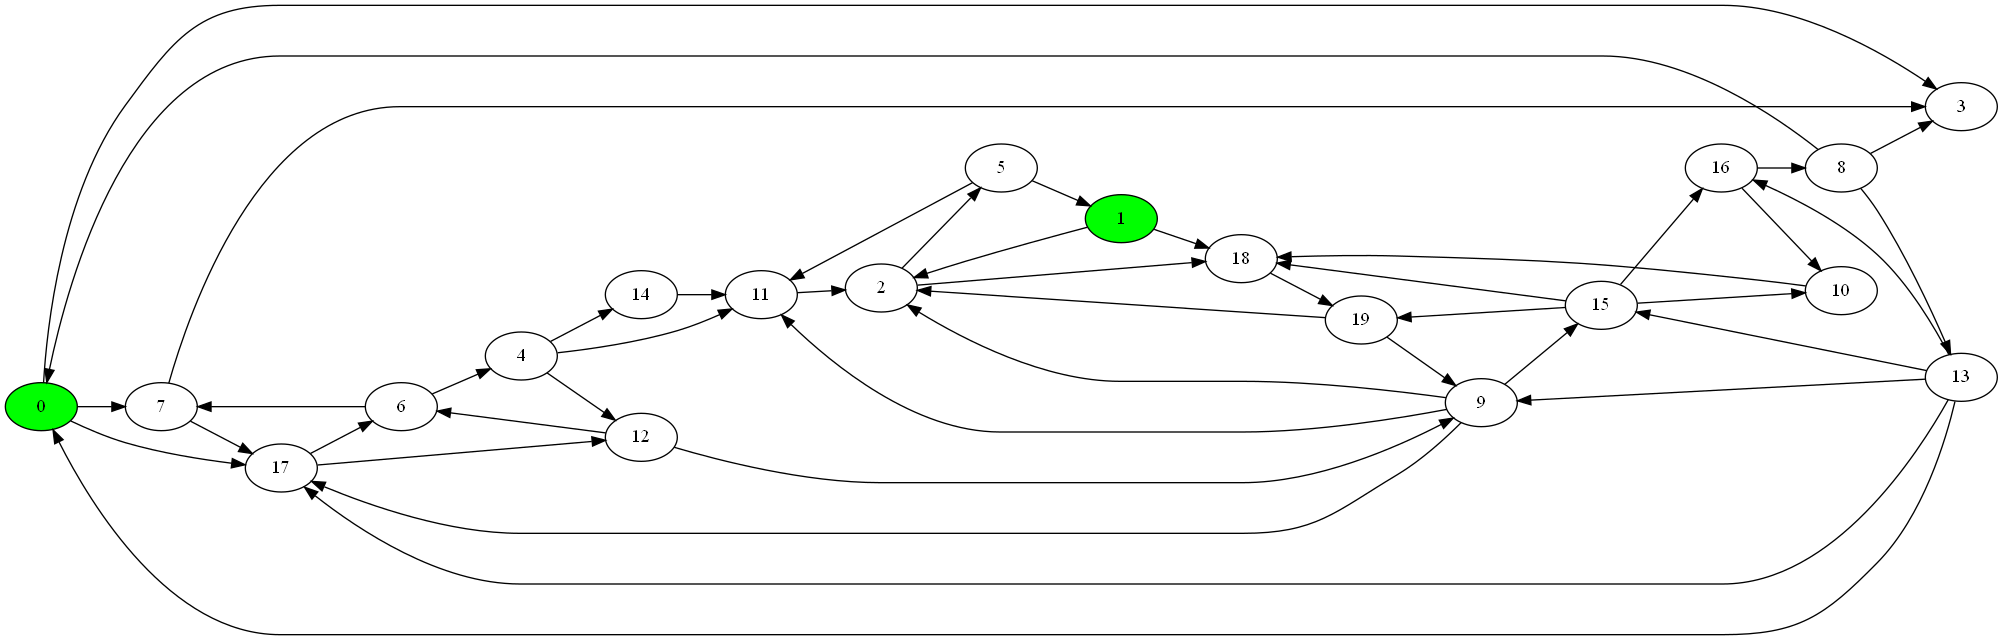
\includegraphics[width=15cm]{../beispielausgaben/huepfburg0.png}
          \caption{Ausgangsgraph 0}
          \label{fig:Ausgangsgraph0}
        \end{figure}
        \lstinputlisting[caption=Ausgabe Beispiel 0]{../beispielausgaben/huepfburg0.out}
        \begin{figure}[H]
          \centering
          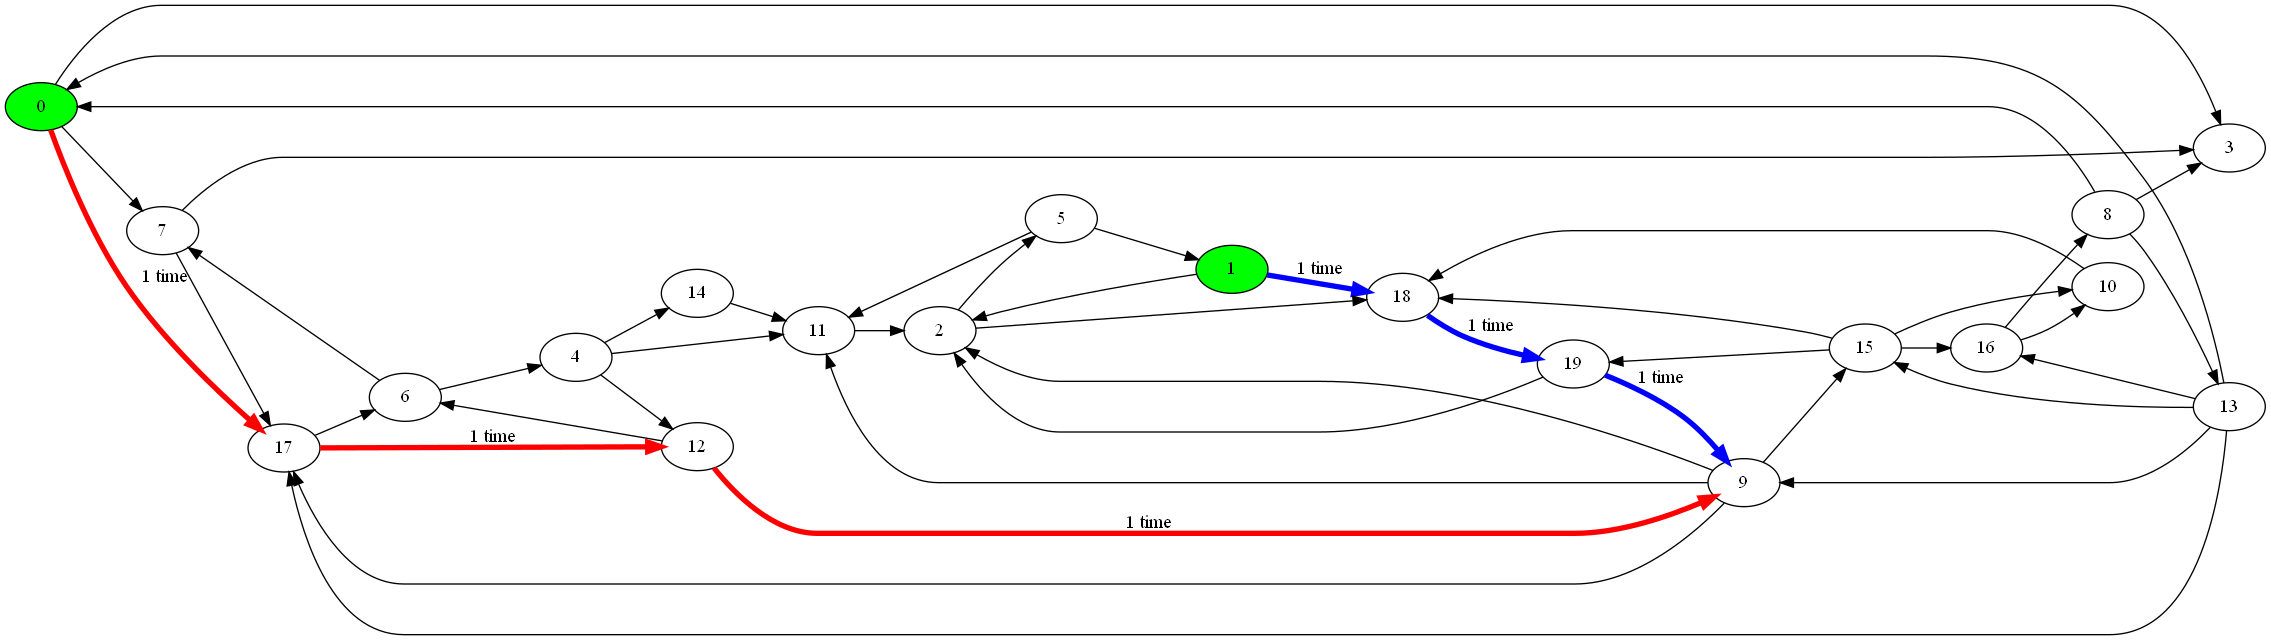
\includegraphics[width=15cm]{../beispielausgaben/huepfburg0_end.png}
          \caption{Endgraph 0}
          \label{fig:Endgraph0}
        \end{figure}

      
      \subsubsection{Beispiel 1}
        \begin{figure}[H]
          \centering
          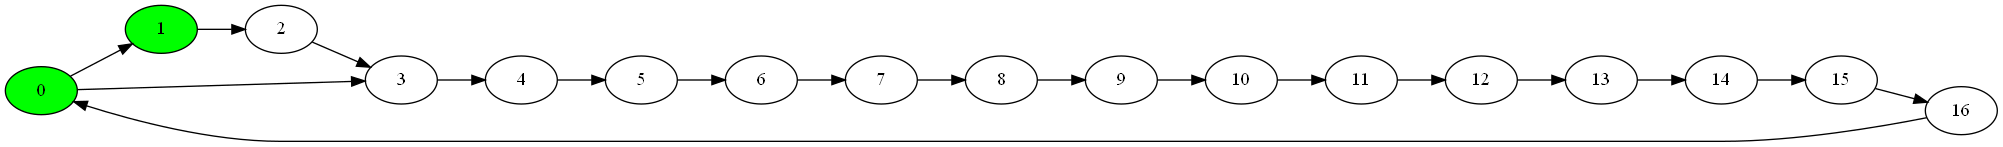
\includegraphics[width=15cm]{../beispielausgaben/huepfburg1.png}
          \caption{Ausgangsgraph 1}
          \label{fig:Ausgangsgraph1}
        \end{figure}
        \lstinputlisting[caption=Ausgabe Beispiel 1]{../beispielausgaben/huepfburg1.out}
        \begin{figure}[H]
          \centering
          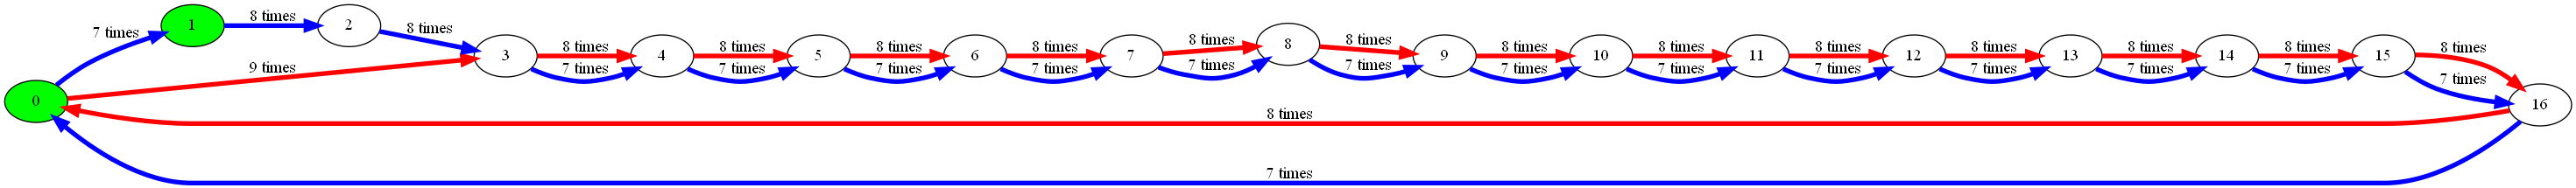
\includegraphics[width=15cm]{../beispielausgaben/huepfburg1_end.png}
          \caption{Endgraph 1}
          \label{fig:Endgraph1}
        \end{figure}


      \subsubsection{Beispiel 2\label{sec:Beispiele:2}}
        \lstinputlisting[caption=Ausgabe Beispiel 2]{../beispielausgaben/huepfburg2.out}
        \begin{figure}[H]
          \centering
          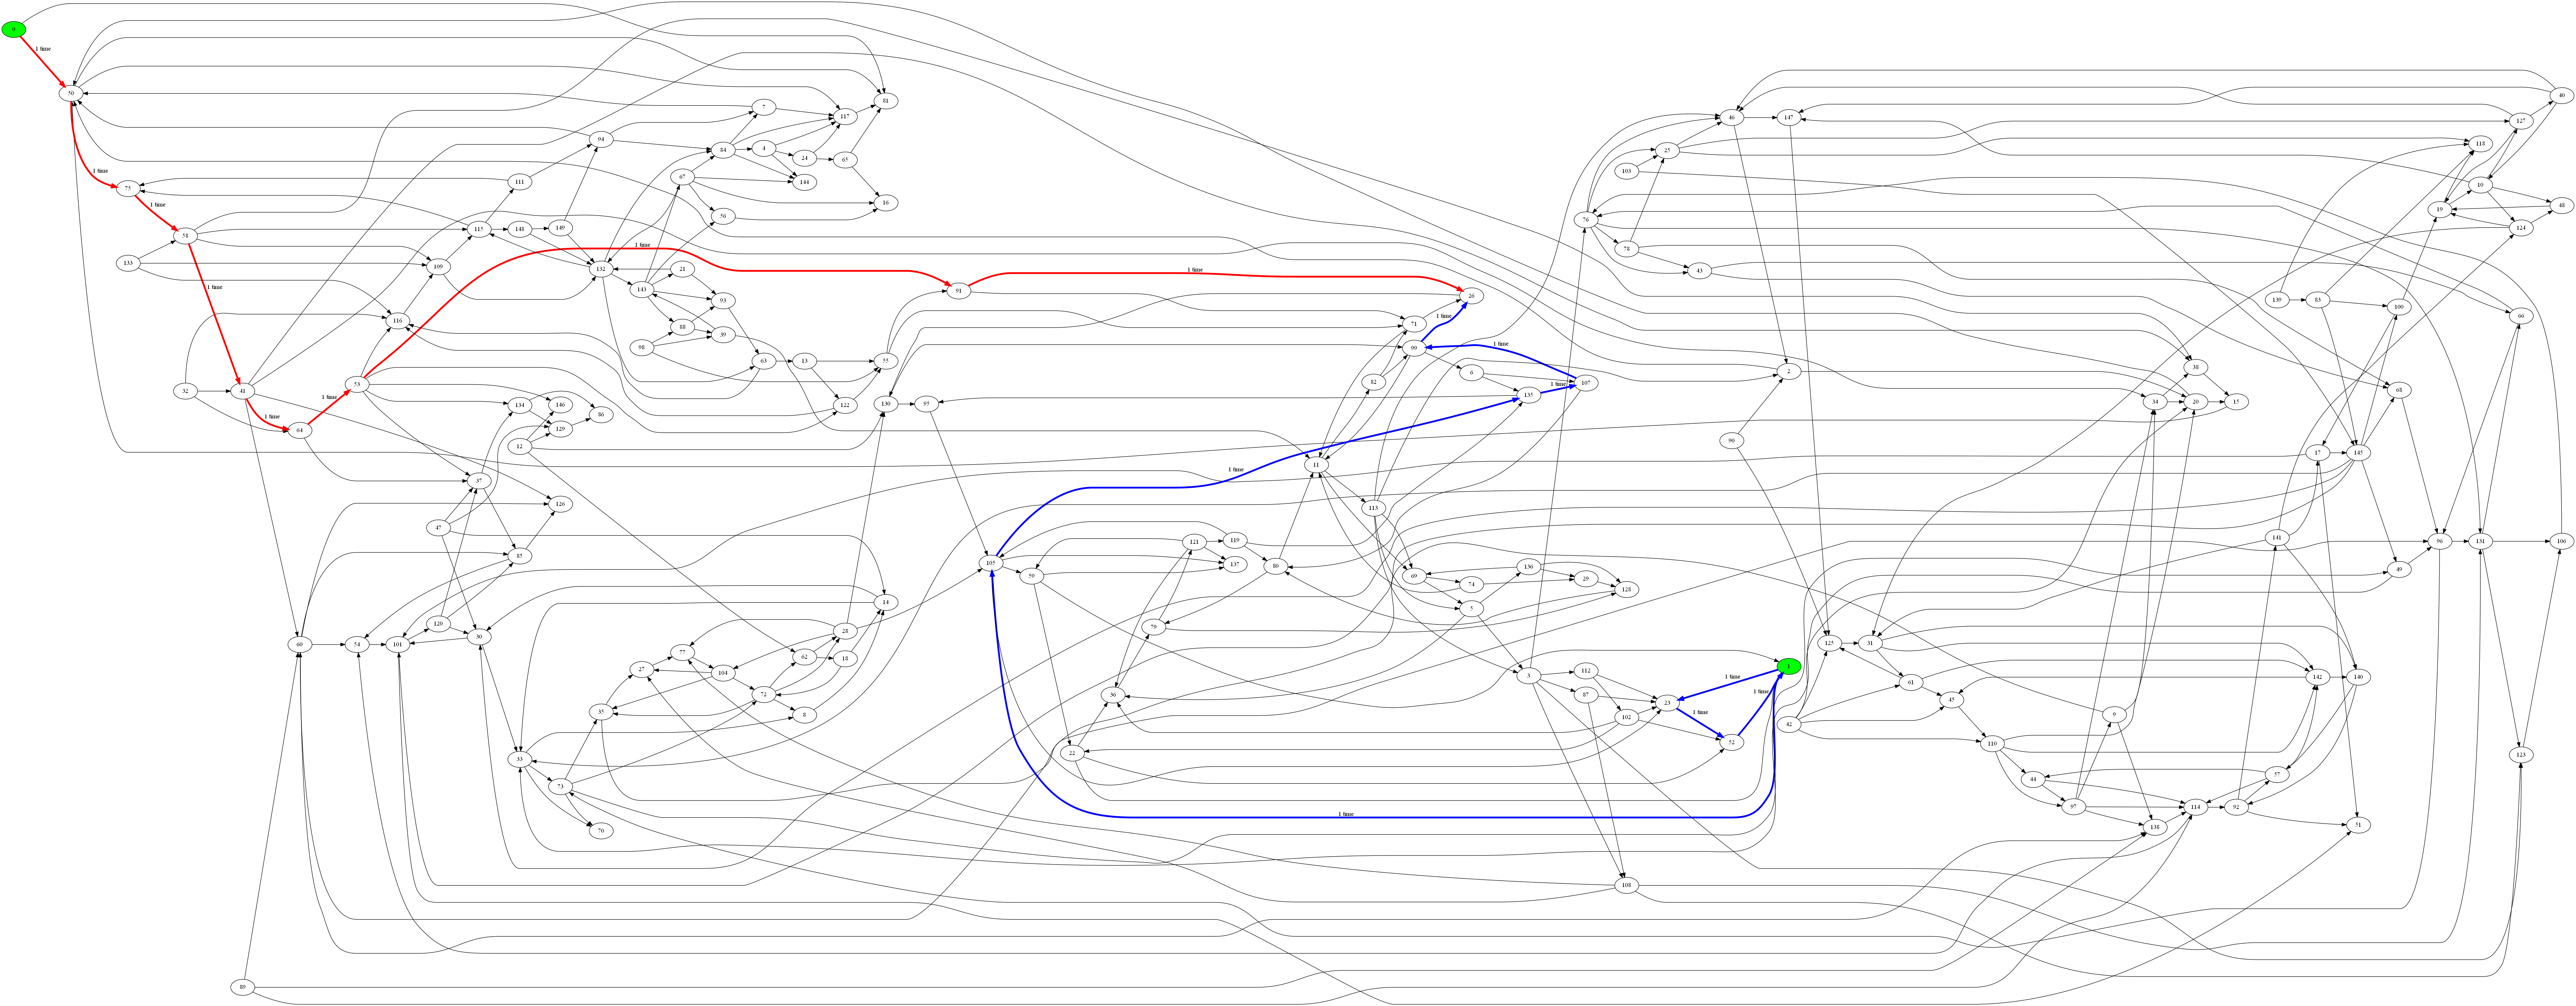
\includegraphics[width=15cm]{../beispielausgaben/huepfburg2_end.png}
          \caption{Endgraph 2}
          \label{fig:Endgraph2}
        \end{figure}

      \subsubsection{Beispiel 3}
        \begin{figure}[H]
          \centering
          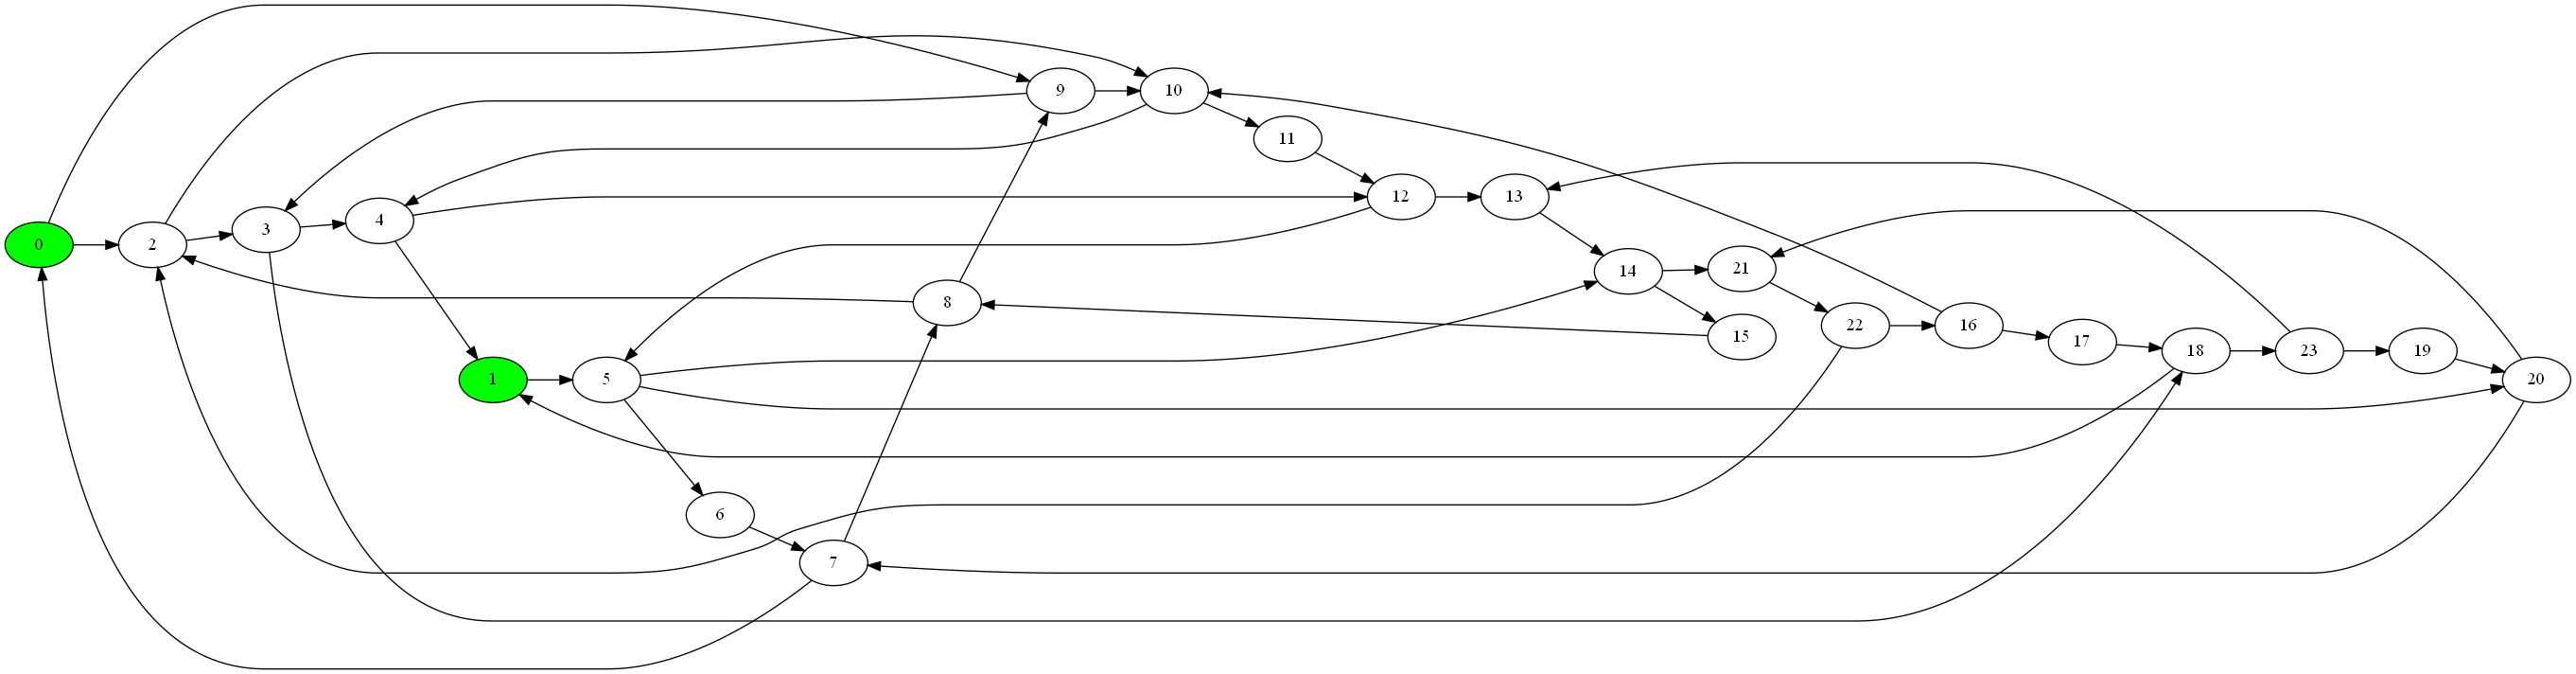
\includegraphics[width=15cm]{../beispielausgaben/huepfburg3_end.png}
          \caption{Ausgangsgraph 3}
          \label{fig:Ausgangsgraph3}
        \end{figure}
        \lstinputlisting[caption=Ausgabe Beispiel 3]{../beispielausgaben/huepfburg3.out}

      \subsubsection{Beispiel 4}
        \lstinputlisting[caption=Ausgabe Beispiel 4]{../beispielausgaben/huepfburg4.out}
        \begin{figure}[H]
          \centering
          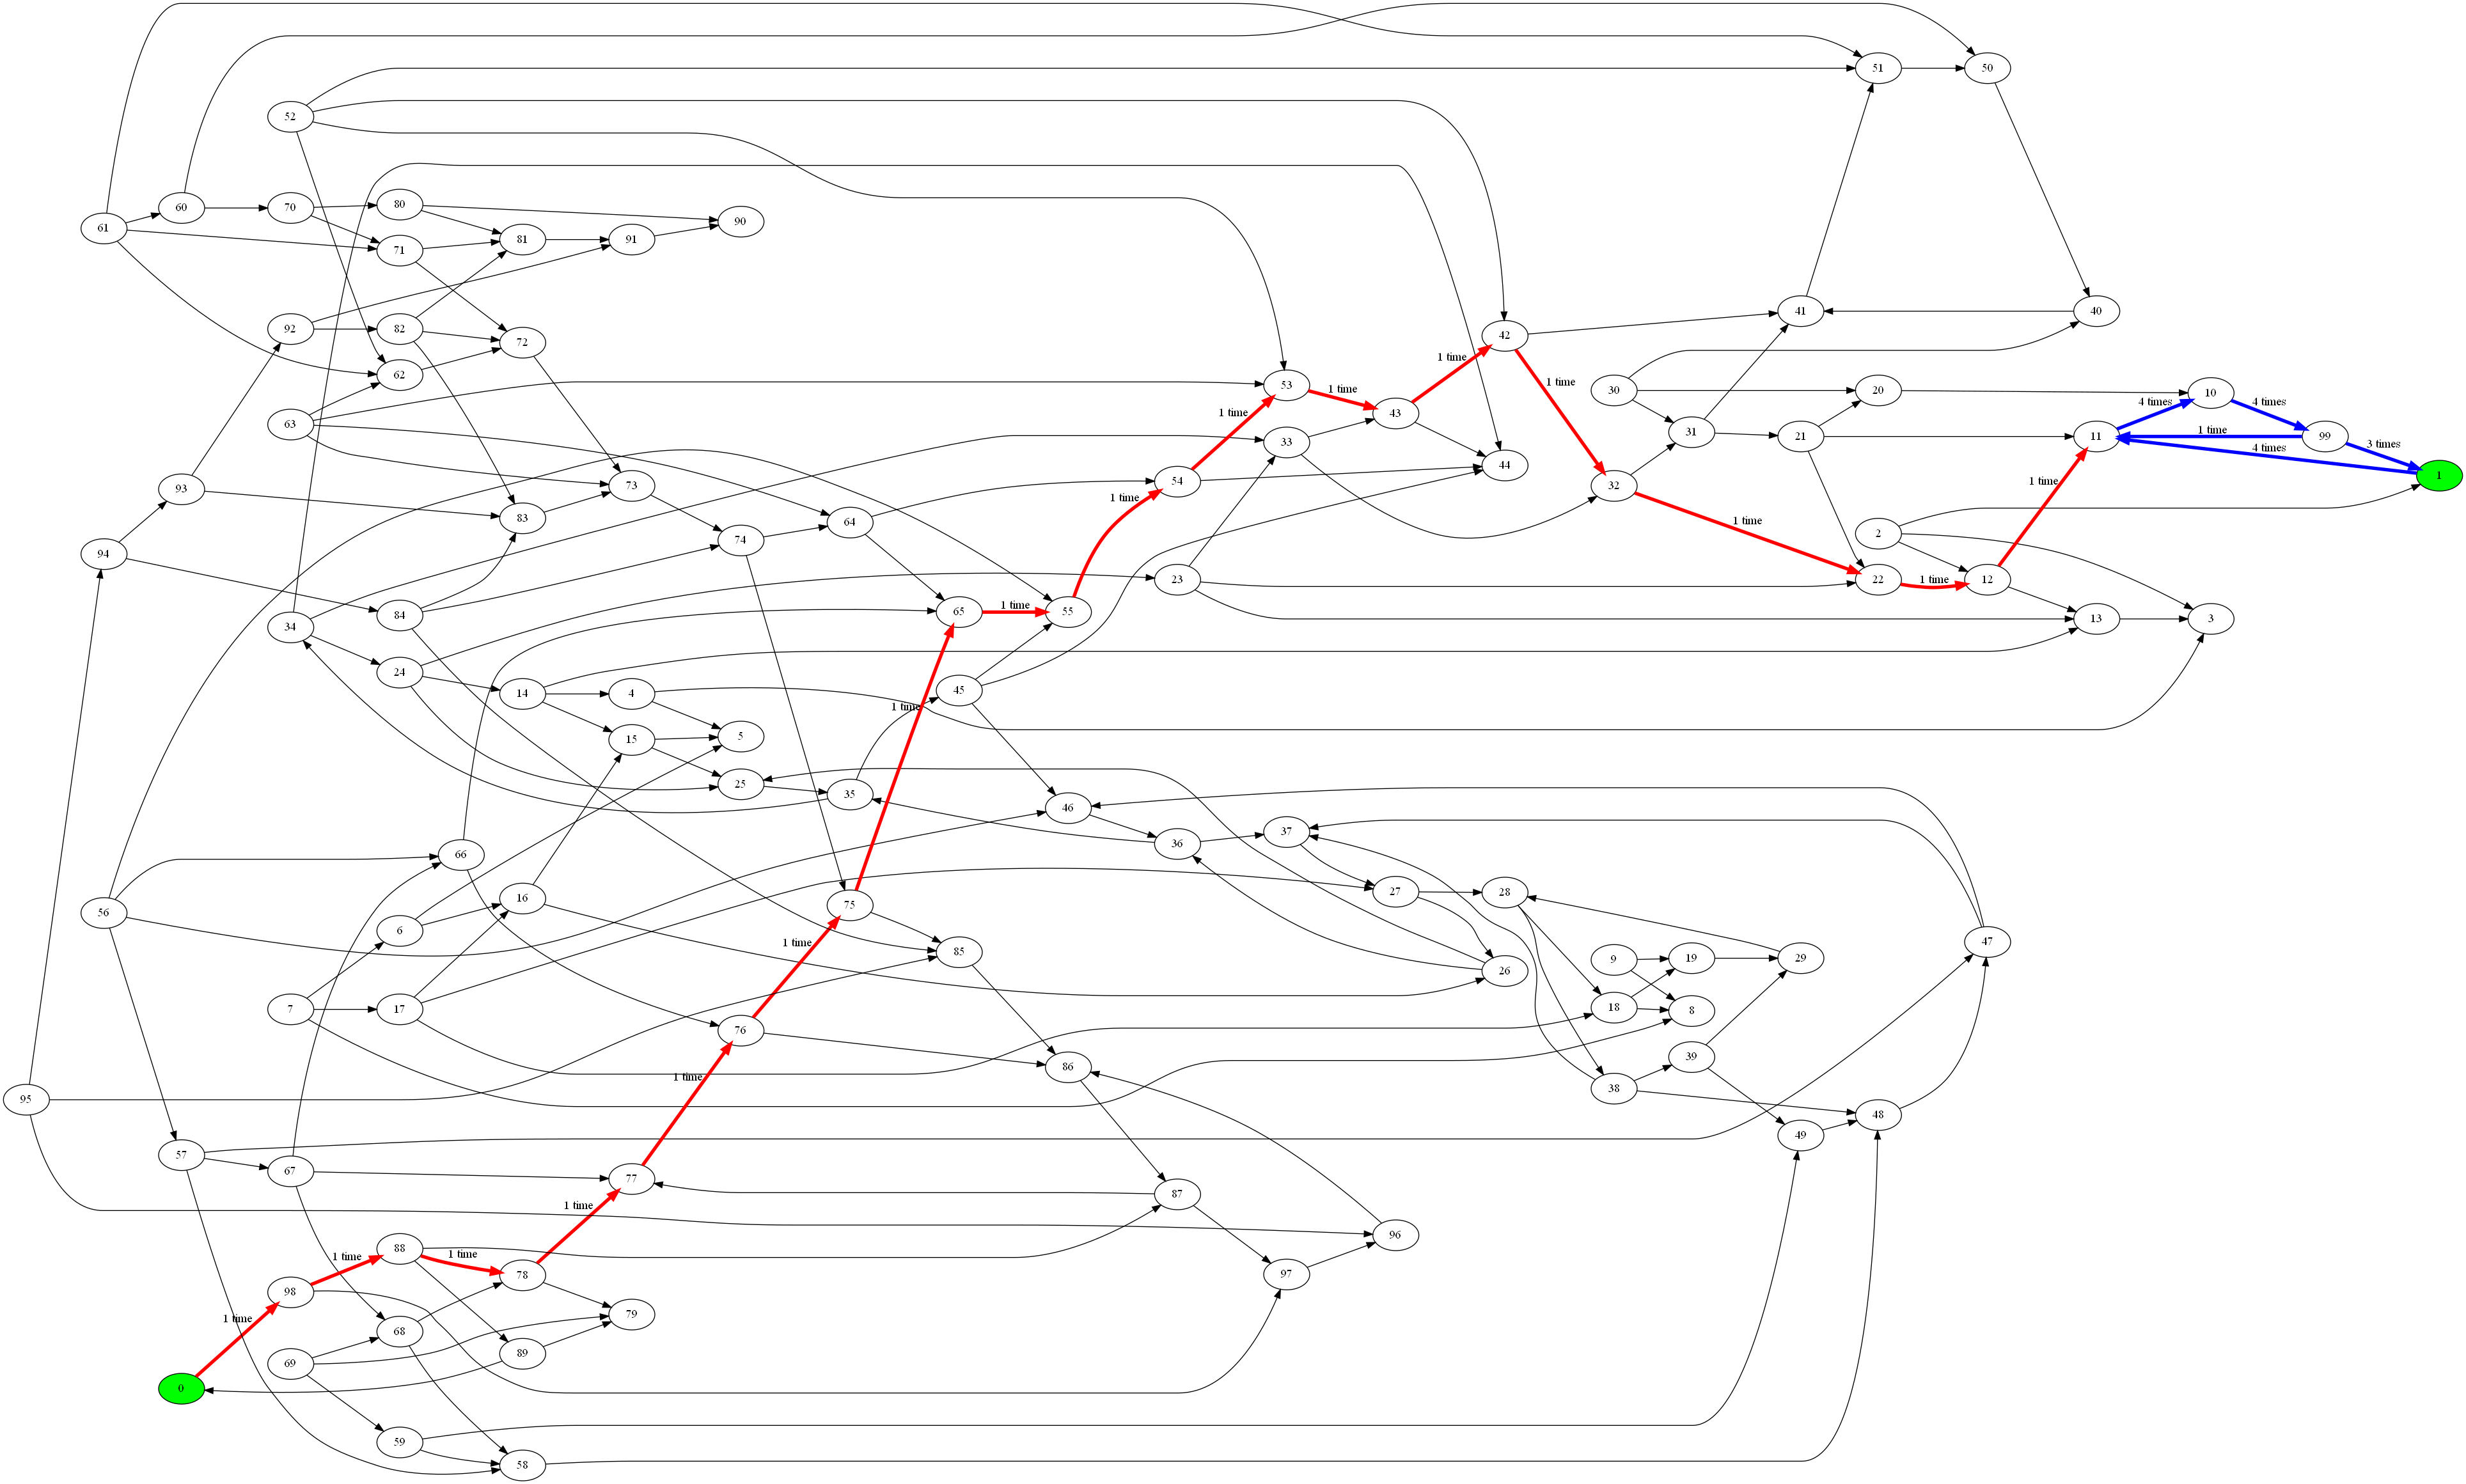
\includegraphics[width=15cm]{../beispielausgaben/huepfburg4_end.png}
          \caption{Endgraph 4}
          \label{fig:Endgraph4}
        \end{figure}

    \subsection{Eigene Beispiele}
      
      \subsubsection{Beispiel 5}
        \begin{figure}[H]
          \centering
          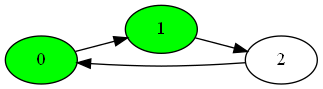
\includegraphics[width=5cm]{../beispielausgaben/huepfburg5.png}
          \caption{Ausgangsgraph 5}
          \label{fig:Ausgangsgraph5}
        \end{figure}

        \lstinputlisting[caption=Ausgabe Beispiel 5]{../beispielausgaben/huepfburg5.out}
        
  %% ___ Quellcode ___ %%
  \section{Quellcode}
    \lstinputlisting[language=C++]{../source/Aufgabe_5.cpp}
\end{document}